\chapter{Introduction}

As the information around us grow exponentially, spatial context about such information is becoming more and more important and useful. For example, If one wants to go from one place to other, He or she always chooses the path that is spatially shortest. Another good spatially aware example is when a person wants to buy a house. Many factors affecting the decision to buy a house are inherently spatially aware, like how far is the hospital, how far is the school facility or is there any good restaurants available nearby. All these examples suggests that one of the crucial factor while buying a house is how qualitative is the spatial neighbourhood. Or we can say that many decisions occurring in everyday life of a person are spatially aware.
\newline
\par
It can be said that spatial data is another dimension for organizing information. With this, getting and organizing spatial data for yielding useful information becomes more and more useful. This creates a desired motivation for building such system to effectively collect and utilize spatial data.


\section{Motivation}
Currently available search engines are good for normal data such as text and web links, but when it comes to searching and ranking spatial data, none of the currently available search engines can provide efficient results. One of the reason for this can be that not all Geo-spatial data is publicly available. Other problems is that repositories containing spatial data are not generally indexed and the meta-data information about what data they contain is not easily available. Also the normally crawled data is not kept in a spatially aware manner. Our motivation here is to build a registry service that can crawl spatial data from the open web, avail data from national government agencies as well as open source free repositories. Once the data is available various kinds of tasks can be built on top of that. This behaves as a foundation platform to provide basic and robust services upon which various other services can be built. We call this as Geo-Service Portal. One can easily build and perform various type of spatial queries like GetMap on the data available. Various graphical applications as well as application programming interfaces(APIs) can be provided on the available data to cater in use in various ways. A query interface can be built upon the data available from catalog service. This query interfaces can provide various views for user specific user queries. An spatial-temporal analytics can also be done using the catalog. Change of data can be tracked. Other use cases can be finding the spread of diseases or getting the area affected by flood. Many other applications can be generated.

\section{Problem Statement}
The aim of this project is to create a foundation platform for crawling, storing, maintaining and publishing meta-data information about spatial data and corresponding providers and to utilize this information to perform efficient query orchestration.


\section{Objectives}

\begin{enumerate}

\item \textbf{Build a topical crawler to crawl the web and store Geo-spatial metadata.}
\par
\indent A topical crawler is a special type of crawler which only searches for information of a particular topic interest. Here the topical crawler crawls the open web, finds and filters URLs found by it. This module checks whether the server provided by the URL is capable of providing OGC compliant geo-spatial web services or not. If the URL is found to be a geo-server it stores all the metadata information about the Geo-server and about the data it contains into the database. It uses domain ontology knowledge to classify data into different domains. This information then later can be utilized to query and find useful information.
\newline
\item \textbf{Build an OGC compliant catalog service to publish and search accumulated metadata.}
\par
The aim here is to build a web service that can query and publish relevant metadata information from the database. The catalog service is real-time. The data stored in the catalog changes with time to reflect changes in corresponding data from the providers. This can also be explored to examine spatio-temporal nature of the data. The catalog service should be built in such a way that queries can be processed in real time. For this purpose the data should be stored in database in structured manner rather than storing it in plain json or XML files. The responses provided by the spatial repositories are generally in XML, GML or shape format, catalog service parses the data to store data in a structured way in database so that various query operations can be supported in OGC compliant manner. One other crucial point for catalog service is to provide high availability. Registry is used to search as well as publish the available data.\\
\begin{figure}[h]
  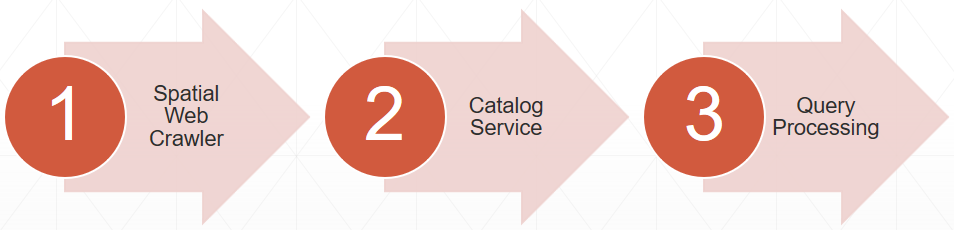
\includegraphics[width=\textwidth]{pix/flow}
  \caption{3 - staged pipeline approach}
\end{figure}
\newline
\item \textbf{Build Query orchestration service to perform real-time query with heterogeneous data sources and cost matrices associated with them.}
\par
One of the tasks of catalog service is to provide relevant information to the querying machine or person. The data that is stored by different repositories can be of heterogeneous form. Task of query orchestration is to find relevant information across all available data sources and perform the query using all relevant data. If the data is available from multiple data sources different type of ranking and cost matrices can be associated to provide most relevant information to the user. Query orchestration is also associated with ranking. While retrieving the data it should be presented to user in a ranked retrieval manner based on some metrics. Here we have discussed two techniques of ranked retrieval and indexing called Quad tree based indexing and ranking based on quality preferences.
\end{enumerate}

\section{Organization of thesis}
This thesis is mainly organized into six chapters. The first chapter gives introduction about the subject matter, it clears the motivation and advantages of the project. It defines the problem statement and states as well as explains the objectives of the project. The second chapter namely literature survey, provides already available data about the subject and proposed solution methods. This section first explains about the data for the model to be work with. It explains the web services and APIs build for spatial data. Then it explains about three part of the foundation platform, Spatial web crawler, Catalog service and query orchestration. Chapter 2 also discusses about the previous work done in the respective fields. 
\newline
\par 
Chapter 3, 4 and 5 are the core foundation blocks for Geo-service portal foundation platform. Chapter 3 is explains about the spatial web crawler. It explains the architecture and the algorithm used for the spatial web crawler. It also explains advantages of spatial web crawler. Chapter 4 contains information about spatial metadata discovery and publishing. It discusses objectives for the catalog service. It also give architecture and implementation details about catalog service for web and query processing. It also shows example results. It also extends the concept to cloud based paradigms.Chapter 5 gives a look into spatial query orchestration. It discusses about two broad strategies two index and rank spatial data.
\newline
\par
The final chapter concludes the morals of the thesis and creates a pathway for better optimizing and extending the proposed solution for the future work.
% \section{Development Platform}